\newpage
\hypertarget{checkCard vis}{}
\subsection{Implementing check}
\visHeader

\begin{itemize}

\vspace{1cm}

\item[$\blacktriangleright$] Since you're nearly a SDM wizard already, try using concepts we have already learnt to create the control flow for
\texttt{Partition::check} as depicted in Fig.~\ref{fig:sdm_check_start}.

\vspace{1cm}

\begin{figure}[htbp]
\begin{center}
  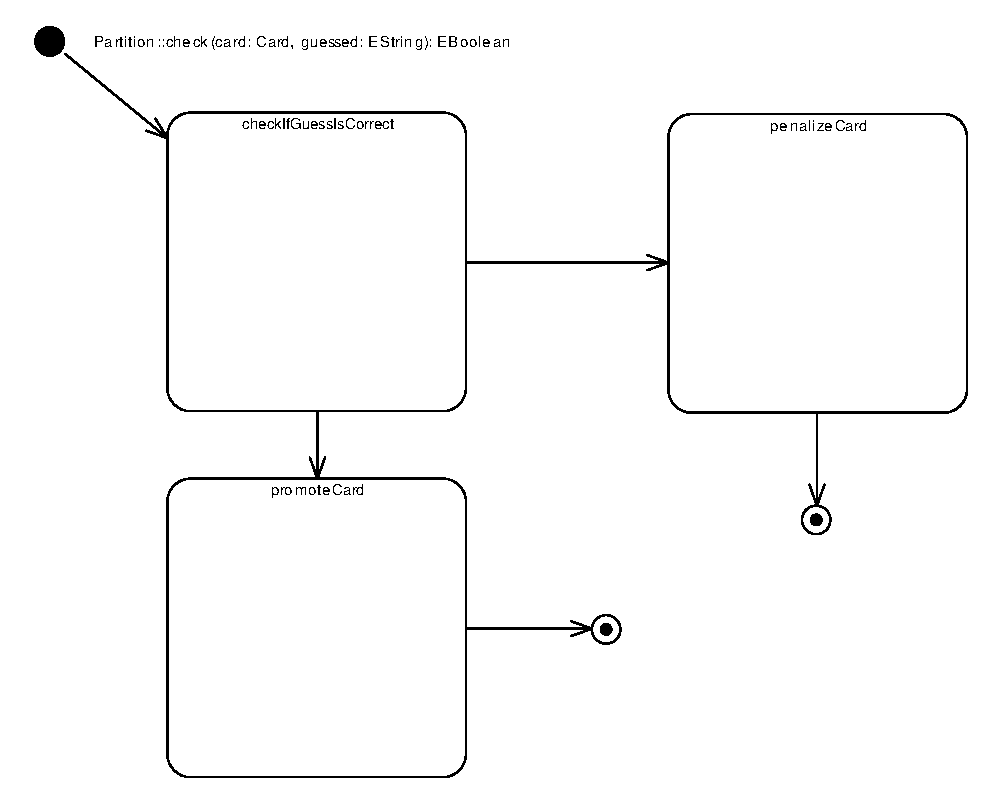
\includegraphics[width=1\textwidth]{ea_activityCheck.pdf}
  \caption{Activity diagram for \texttt{Partition::check}}
  \label{fig:sdm_check_start}
\end{center}
\end{figure}

\vspace{1cm}

\item[$\blacktriangleright$] In \texttt{checkIfGuessIsCorrect}, create an object variable that is bound to the parameter argument, \texttt{card} 
(Fig.~\ref{fig:sdm_check_addCard}). This will represent the card the user picked from the learning box. Remember, the binding for this variable is implicitly
defined when its name is the same as the argument's name.

\begin{figure}[htbp]
\begin{center}
  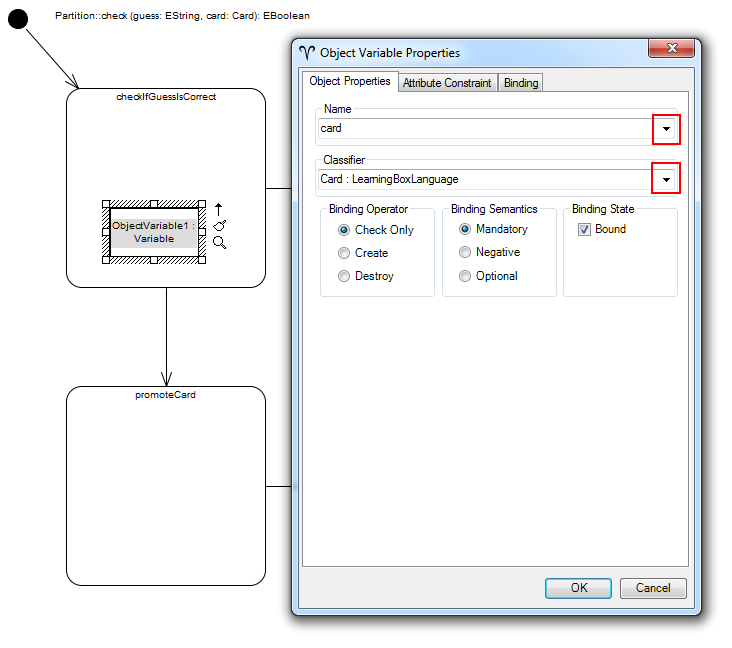
\includegraphics[width=\textwidth]{ea_addObjVarCard}
  \caption{Creating the card variable}
  \label{fig:sdm_check_addCard}
\end{center}
\end{figure}

\clearpage

\item[$\blacktriangleright$] Now that the pattern has the correct card to check, it needs to compare the user's guess against the unseen \texttt{face} value on
the opposite side. To do this, we need to specify an \emph{attribute constraint}. Open the \texttt{attribute constraint} tab as depicted in
Fig.~\ref{fig:sdmcheck_att_constraint}, select the correct object attribute (\texttt{face}) and comparison operator.

\begin{figure}[htbp]
\begin{center}
  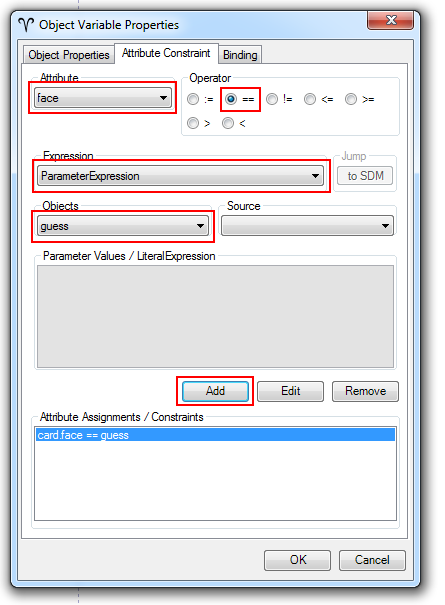
\includegraphics[width=0.6\textwidth]{ea_addAttConst}
  \caption{Creating an attribute constraint}
  \label{fig:sdmcheck_att_constraint}
\end{center}
\end{figure}

\item[$\blacktriangleright$] Similar to how the return value was specified in the previous SDM, set the \texttt{ParameterExpression} to refer to \texttt{guess}.
Press \texttt{Add} and admire your first attribute constraint.

\vspace{1cm}

Before building the other two activity nodes, let's quickly return to the control flow. Currently, the pattern will branch off into two separate patterns after
completing the initial check, then terminate the method based on whichever activity finishes first\ldots and that's not what we want at all! We need to add
\emph{edge guards} to change this into an \emph{if/else} construct based on the results of the comparison.

\newpage

\item[$\blacktriangleright$] To add a guard to the edge leading from \texttt{check\-If\-Guess\-Is\-Correct} to \texttt{penalize\-Card}, double click the edge
and set the \emph{Guard Type} to \texttt{Failure} (Fig.~\ref{fig:sdm_check_guard}).

\vspace{0.5cm}

\begin{figure}[htbp]
\begin{center}
  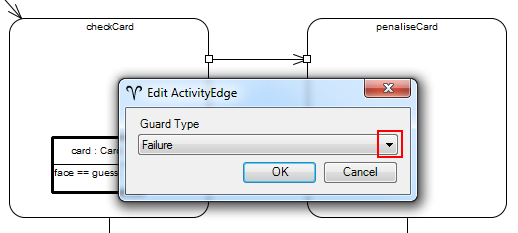
\includegraphics[width=0.75\textwidth]{ea_addTransitionGuard}
  \caption{Add a transition with a guard}
  \label{fig:sdm_check_guard}
\end{center}
\end{figure}

\vspace{0.5cm}

\item[$\blacktriangleright$] Repeat the process for the \texttt{Success} edge leading to \texttt{promoteCard}.

\vspace{0.75cm}

Another feature of eMolfon (with EA) provides a means of coping with large patterns.\footnote{You thought I was going to say `coping
with our coffee addiction', weren't you?} It might be nice to visualise \emph{small} story patterns directly in their nodes, but for large patterns or complex
control flow, such diagrams would get extremely cumbersome and unwieldy very quickly! This is indeed a popular argument against visual languages and it might
have already crossed your mind (``This is cute, but it'll \emph{never} scale!''). With the right tools and concepts however, even huge diagrams can be
mastered. We support \emph{extracting} story patterns into their own diagrams, and unless the pattern is really concise with 2 or 3 object variables, recommend
this course of action.

\vspace{0.5cm}

\item[$\blacktriangleright$] To try this, double-click the \texttt{promoteCard} story node and choose \texttt{Extract Story Pattern}
(Fig.~\ref{fig:sdm_check_extract_storypattern}). Note the new diagram that is immediately opened and created in the project browser
(Fig.~\ref{fig:sdm_new_sub_diagram}).

\begin{figure}[htbp]
\begin{center}
  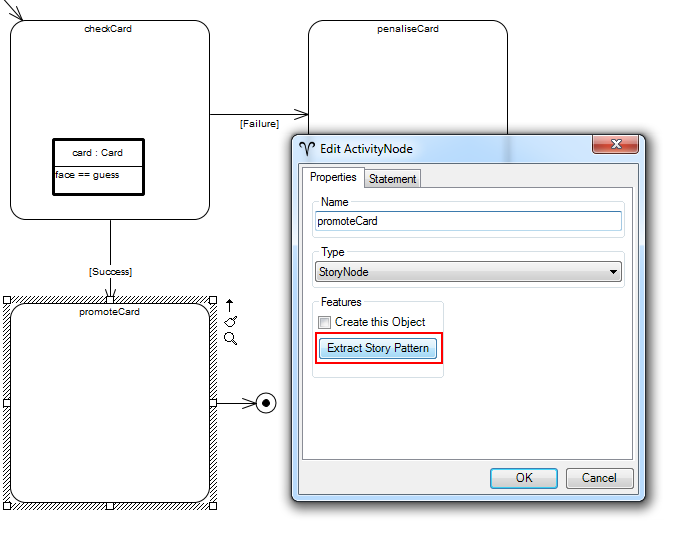
\includegraphics[width=0.8\textwidth]{ea_extractStoryPattern}
  \caption{Extract a story pattern for more space and a better overview}
  \label{fig:sdm_check_extract_storypattern}
\end{center}
\end{figure}

\begin{figure}[htbp]
\begin{center}
  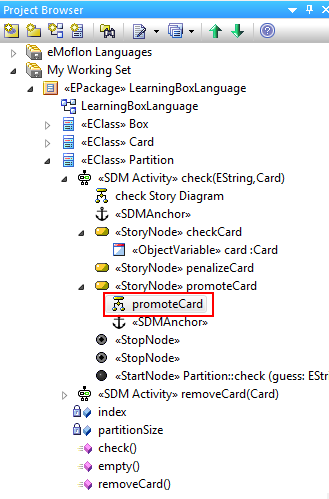
\includegraphics[width=0.45\textwidth]{sdm_promoteCardProjBrowser}
  \caption{A new sub diagram is created automatically}
  \label{fig:sdm_new_sub_diagram}
\end{center}
\end{figure}

\newpage

Another EA gesture you should start to take advantage of is a good ol' \emph{Drag and Drop} action from the project browser\footnote{Remember he other two
gestures we have learnt: ``Quick Link'' and ``Quick Create''} into a diagram. We can use this move as an alternative to creating new objects (with known types) from the SDM
toolbox.

\vspace{0.5cm}

\item[$\blacktriangleright$] To create a new \texttt{Card} object variable, simply drag and drop the class from the project browser into the new (extracted)
pattern diagram (Fig.~\ref{fig:sdm_check_bound_card}).

\begin{figure}[htbp]
\begin{center}
  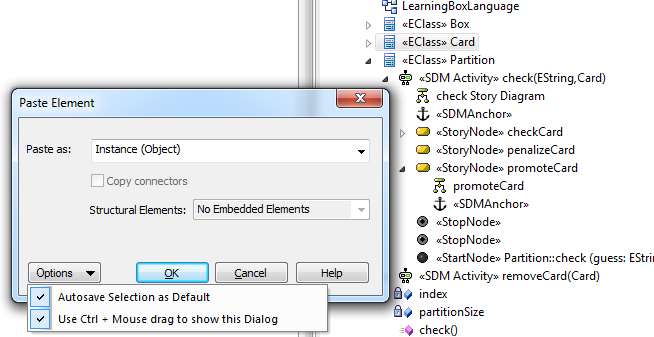
\includegraphics[width=0.8\textwidth]{ea_dragDropDialogue}
  \caption{Add a new object variable per drag and drop}
  \label{fig:sdm_check_bound_card}
\end{center}
\end{figure}

\item[$\blacktriangleright$] A dialogue will appear asking what kind of variable should be created. You can create (1) a simple link (which would
refer to and be represented by \texttt{Card}'s class), (2) create an instance of \texttt{Card} as an object, or (3) create a subclass. Paste \texttt{Card} as an
instance and check \texttt{Autosave Selection as Default} under ``Options" so option (2) will be used next time by default. You should also check \texttt{Use
Ctrl + Mouse drag to show this Dialog}, so this dialogue doesn't appear every time. Don't worry - if you ever need options (1) and (3), you  just need to hold
\texttt{Ctrl} when dragging to invoke the dialogue then change the settings.

\vspace{0.5cm}

\item[$\blacktriangleright$] After creating the object, the same object properties dialogue will open.  Set the \texttt{Name} to \texttt{card} and its
\texttt{Binding State} to \texttt{Bound} (Fig.~\ref{fig:sdm_new_card_properties}).

\newpage

\begin{figure}[htbp]
\begin{center}
  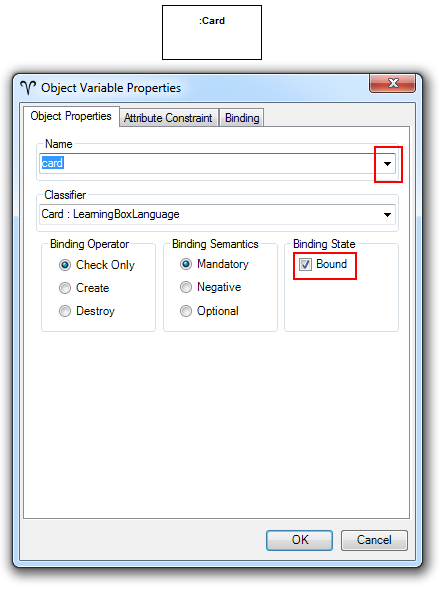
\includegraphics[width=0.5\textwidth]{ea_addBoundObj}
  \caption{Object variable properties of the new card}
  \label{fig:sdm_new_card_properties}
\end{center}
\end{figure}

The main advantage of drag and drop is that the \texttt{Object Variable Pro\-per\-ties} dialogue should have the type of the object pre-configured. Choosing
the type in the project browser and dragging it in is (for most people) a more natural gesture than choosing the type from a long drop-down menu (as we had to
when using the SDM toolbar). This can be a great time saver for large metamodels\footnote{Drag and drop is also possible in embedded story patterns
(still visualised in their story nodes).  You must ensure however, that the object variable is \emph{completely} contained inside the story node and does not
stick out over any edge}.

\vspace{0.5cm}

\item[$\blacktriangleright$] Currently, we have the single \texttt{card} that we want to promote through the box. Drag and drop two further object variables for
the current partition, \texttt{this}, and the \texttt{nextPartition} as depicted in Fig.~\ref{fig:sdm_check_complete_sp}.

\begin{figure}[htbp]
\begin{center}
  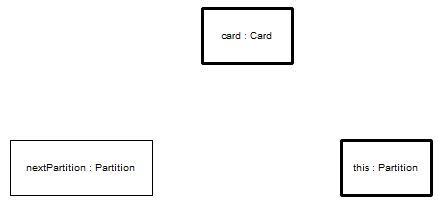
\includegraphics[width=0.8\textwidth]{ea_promoteCardVariables}
  \caption{All object variables for story pattern \texttt{promoteCard}}
  \label{fig:sdm_check_complete_sp}
\end{center}
\end{figure}

\vspace{0.5cm}

An important point to note here is that \texttt{this} and \texttt{card} are visually differentiated from \texttt{nextPartition} by
their bold border lines. This is how we differentiate \emph{bound} from \emph{unbound} (\emph{free}) variables. We already know that matches for bound
variables are completely determined by the current context. On the other hand, matches for unbound variables, have to be determined by the pattern matcher. Such
matches are ``found'' by navigating and searching the current model for possible matches that satisfy all specified constraints (e.g. type of the variable,
links connecting it to other variables and attribute constraints). In our case, the next partition will have to be determined by navigating from \texttt{this}
via the \texttt{next} link in the metamodel.

\vspace{0.5cm}

\item[$\blacktriangleright$] Quick link from \texttt{this} to \texttt{nextPartition} (or vice-versa) to create a \texttt{next} link variable, as shown in
Fig.~\ref{fig:sdm_check_link_variable}. As you can see, there are several more property options. The goal is to have the current partition to proceed or point
to the \texttt{nextPartition} via the \texttt{next} reference, so select the second option. This will cause the reference to be defined in \texttt{this}.
Alternatively, you could define the reference in \texttt{nextPartition} by setting the link proceed from the next partition into the \texttt{previous}
partition, \texttt{this}.

\begin{figure}[htbp]
\begin{center}
  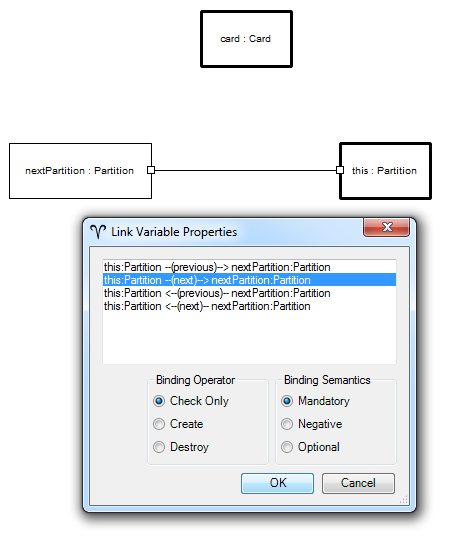
\includegraphics[width=0.85\textwidth]{ea_promoteLinkProperties}
  \caption{Connecting \texttt{this} and \texttt{nextPartition}}
  \label{fig:sdm_check_link_variable}
\end{center}
\end{figure}

\vspace{0.5cm}

\item[$\blacktriangleright$] Continue creating links between \texttt{card} and each partition. Remember - you want to \emph{destroy} the reference to
\texttt{this}, and \emph{create} a new connection to \texttt{nextPartition}. If everything is set up correctly, \texttt{promoteCard} should now closely resemble
Fig.~\ref{fig:sdm_check_complete_activity_node}.

\begin{figure}[htbp]
\begin{center}
  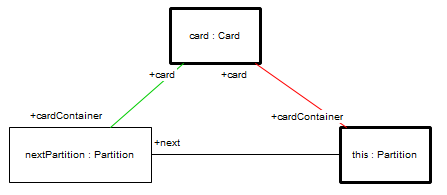
\includegraphics[width=0.8\textwidth]{ea_promoteCardCompleted}
  \caption{Complete story pattern for \texttt{promoteCard}}
  \label{fig:sdm_check_complete_activity_node}
\end{center}
\end{figure}

\clearpage

\item[$\blacktriangleright$] Double click the anchor in the top left corner and repeat the process for \texttt{penalizeCard}: First extract the story pattern,
then create the necessary variables and links as depicted in Fig.~\ref{fig:sdm_check_complete_penalize}. As you can see, this pattern is nearly identical to
\texttt{promoteCard}, except it moves the card to a \texttt{previousPartition}.

\vspace{0.5cm}

\begin{figure}[htbp]
\begin{center}
  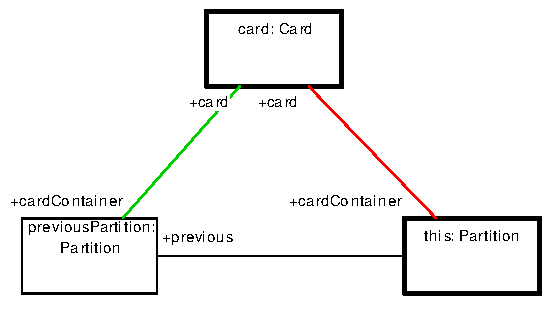
\includegraphics[width=0.8\textwidth]{ea_completeActivityPenalize.pdf}
  \caption{Story pattern for activity node \texttt{penalizeCard}}
  \label{fig:sdm_check_complete_penalize}
\end{center}
\end{figure}


\vspace{0.5cm}

To complete the \texttt{check} SDM, we need to signal (as a return value) the result of the check - was the card promoted or penalised? To do this, we need to
edit the stop nodes so they return a\define{LiteralExpression}\emph{LiteralExpression}. This expression type can be used to specify arbitrary text, but
should really only used for true literals like 42, ``foo'' or \texttt{true}. It can be (mis)used for formulating any (Java) expression that will simply be
transferred ``literally'' into the generated code, but this is obviously sort of dirty\footnote{It defeats, for example, any attempt to guarantee type safety}
and should be avoided when possible.

\item[$\blacktriangleright$] To implement a literal, double click the stop node stemming from  \texttt{promoteCard}, and change the expression type from
\texttt{void} to \texttt{LiteralEx\-pression} (Fig.~\ref{fig:sdm_check_literal_exp}). Change the value in the window below to \texttt{true}. Press \texttt{OK},
then finish the SDM by returning \texttt{false} after \texttt{penaliseCard} in the same manner. Your diagram should now resemble
Fig.~\ref{fig:sdm_check_finish}.

\begin{figure}[htbp]
\begin{center}
  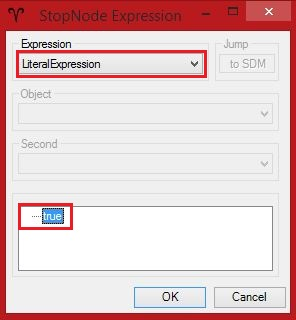
\includegraphics[width=0.5\textwidth]{ea_stopNodeLiteral}
  \caption{Add a return value with a literal expression}
  \label{fig:sdm_check_literal_exp}
\end{center}
\end{figure}

\begin{figure}[htbp]
\begin{center}
  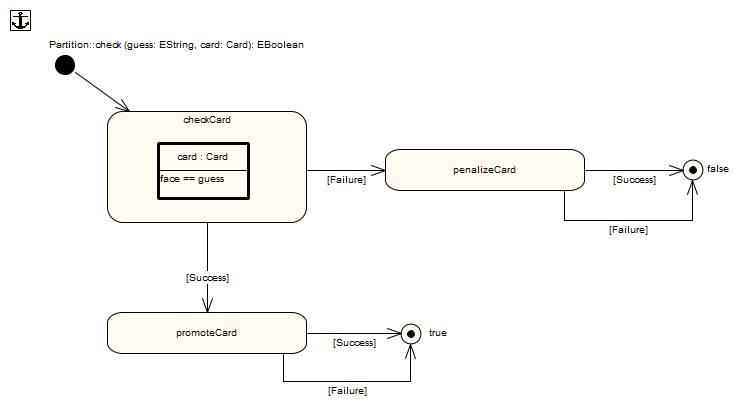
\includegraphics[width=\textwidth]{ea_sdmCheckComplete}
  \caption{Complete SDM for \texttt{Partition::check}}
  \label{fig:sdm_check_finish}
\end{center}
\end{figure}

\clearpage

\item[$\blacktriangleright$] Great job - the SDM is now complete! Validate and export your project, then inspect the implementation code for \texttt{check}. We
strongly recommend that you even write a simple JUnit test (take a look at our simple test case from Part I for inspiration) to take your brand new SDM for a
test-spin.

\item[$\blacktriangleright$] To see how this is implemented in the textual syntax, see Figs. \ref{fig:completedPatterns} and \ref{fig:finalMethod} in the
following section.

\fancyfoot[R]{ $\triangleright$ \hyperlink{sec:emptyPartition}{Next}}

\end{itemize}
